\chapter{Introduction}

Game theory is a set of analytical tools and solution concepts, which provide
explanatory and predicting power in interactive decision situations, when the
aims, goals and preferences of the participating players are potentially in
conflict, Szabo and Fath (2007)(ref.). The Prisoner's Dilemma(PD) is a well
known example in Game Theory and in recent years has become the gold standard of
understanding evolution of co-operative behavior \parencite{Lorberbaum1994}. Thus, it
has been a topic of focus in various fields, such as biology, sociology, ecology
and psychology.

In the example of the Prisoner's Dilemma(PD) two criminals have been arrested
and interrogated, with no way of communicating, by the police. They are given
only two choices, to either cooperate with each other or to defect.  Now let us
consider that the prisoner's would be put back to their cells and would be asked
the same question tomorrow. Furthermore, let this happen repeatably. This is
referred to as the Iterated Prisoner's Dilemma(IPD) an example that has been a
rich source of research material since the 1950s but has earned much interest in
the 1980s due to the work done by the political scientist Robert Axelrod(ref.).

In 1980, Axelrod held the first ever IPD computer tournaments (ref), he invited
academics from various fields to submit their strategies in computer code. The
tournaments were of a round robin topology and the first one included sixteen
strategies and the second one sixty-two. In both tournaments the strategy Tit
for Tat was announced the winner and for many years it  was consider to be the
most successful strategy. A large volume of literature merge on the topic
afterwards, also criticism about the initial tournaments. Scientist question
whether the conditions that the first tournament took place favored
tit for tat. An argument was that the initial tournaments thought they included
a small change pf misepercepion it did not examine noise. Noise is the probability
that the player will submit the wrong move. Bendor, Kramer and Stout 1991 (ref.)
stated that TFT performed rather poorly when noise was introduced in the tournament.
Another aspect, is the payoff matrix which according to Kretz 2011 (ref.)
the precise choice of the payoff matrix is relevant to the results.
%I kept the extra things I have written here like I told you. Let me know if
%the gap between Axelrod to Nowak is still big.

Furthermore, another aspect needed to be taken into account was a different
tournament topology. In Evolutionary Games and Spatial Chaos Nowak and May 1992
(ref.)
introduced the spatial topology. In which the nodes represent players, and the
edges, connecting the nodes, refer to the connection between the corresponding
players. Their tournament considered the PD and the players could only defect or cooperate.
They provided proof that cooperative behavior can emerge from a PD tournament in
spatial topology. Many works on the IPD and spatial tournament were held due to
their original paper. Such as (ref.).
These tournaments use either the PD or IPD and simple to complex strategies.
 %can i reference the thesis of Maciver?

One can argue that the real life interactions are more like the spatial ones
because in real life no all players - companies interact with all the opponents.
Additionally, an interest aspects of the spatial topology are the results compared
to those of a round robin one. This dissertation will be focusing on reproducing
a spatial tournament with some of the most successful strategies of various
tournaments that have been held. For the spatial topology it will use various
graphs compared to other works done only using lattices.Concluding how spatial
topology, with any given graph, affects the effectiveness of these strategies.

\section{The Prisoner's Dilemma}

The PD was originally formulated by Merril M. Flood and Melvin Dresher,
who were working on the Flood-Desher Experiment at the RAND cooperation in 1950.
% include a reference
Later in 1950, the mathematician Albert W. Tucker presented the first formal
representation of the PD, titled  A Two-Person Dilemma in a seminar at
Stanford University \parencite{Gass005}.

A description of the PD, found in \parencite{Li2011} is as follows:
There are two players that simultaneously have to decide to whether Cooperate (C)
or Defect (D) with each other, without exchanging information.

\begin{itemize}
  \item If both players choose to cooperate they will both receive a reward (R)
  \item If a player defects and the other cooperates then the defector receives
  a temptation payoff (T) and the cooperator a sucker payoff (S)
  \item If both players defect they will both receive a penalty (P)
\end{itemize}

Fig. 1 illustrates the payoffs matrix.~\ref{fig:pd_payoff}.

\begin{figure}[h!]
\centering
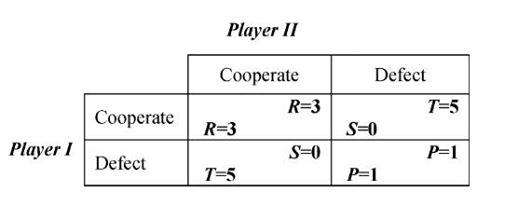
\includegraphics[scale=0.45]{pd_payoff.jpg}
\caption{The payoff matrix for the Prisoners Dilemma \parencite{Li2011}}
\label{fig:pd_payoff}
\end{figure}

Taking into account the assumptions that both players are both rational human
beings \footnote{Players that are rational and will strive to maximize
their payoffs in the game.}
and that there is no way of communication between them. No matter what the
other player does, defecting will be their dominant choice as it yields a higher
payoff than cooperation.
Thus the pure Nash Equilibrium exists when both players defect.Even though, both
players would do better if they were to cooperate.

Furthermore, for this to hold there are some extra assumptions for the relationship
of the four outcomes. The T temptation to defect has to offer the highest payoff for
a player and the worst he could get has to be the sucker S. Likewise, the
reward for mutual cooperation should exceed that of mutual defection P. Thus the
next condition is (ref.):
\begin{equation}
 T > R > P > S
\end{equation}
Moreover, it is assumed that the average of T and S is less than the reward for
mutual cooperation (ref.) :
\begin{equation}
R > 1/2(T+S)
\end{equation}

Same conditions such as rationality, no communication and (1.1), (1.2) apply for
the IPD. An IPD is nothing more than a PD were the players interact for a known
number of times.

\section{Problem Description}

Axelrod's tournaments set a seed for generations of tournaments in the Prisoner's
using computer modeling. Research has shown that by altering the environment of
a tournament the effectiveness of some strategies can change radically. An aspect
that has been investigated as to how the tournament results can bee affected was
the topology. Nowak and May introduced the spatial topology only to set yet another
seed in the PD tournaments. Even so, spatial topology still has not been fully
explored with only a small number of papers focusing on this specific topology.
A goal of this dissertation is to understand the current state of the art in
spatial prisoner’s dilemma tournaments.

The contemporary world is full of networks, according to Maschler 2012. That is
one of the main reasons this dissertation will be focusing on such
topology. Work done at this point consider spatial topology to be that of a square
lattice were each edge represents a player which interacting/playing with only
his neighbors in their von Neuman or Moore's neighborhood. A von Neuman neighborhood
comprises the four cells orthogonally surrounding a central cell where the
Moore's neighborhood eight cells. As shown in Figure :
\begin{figure}[h]
\centering
    \begin{subfigure}[t]{0.40\textwidth}
    \centering
        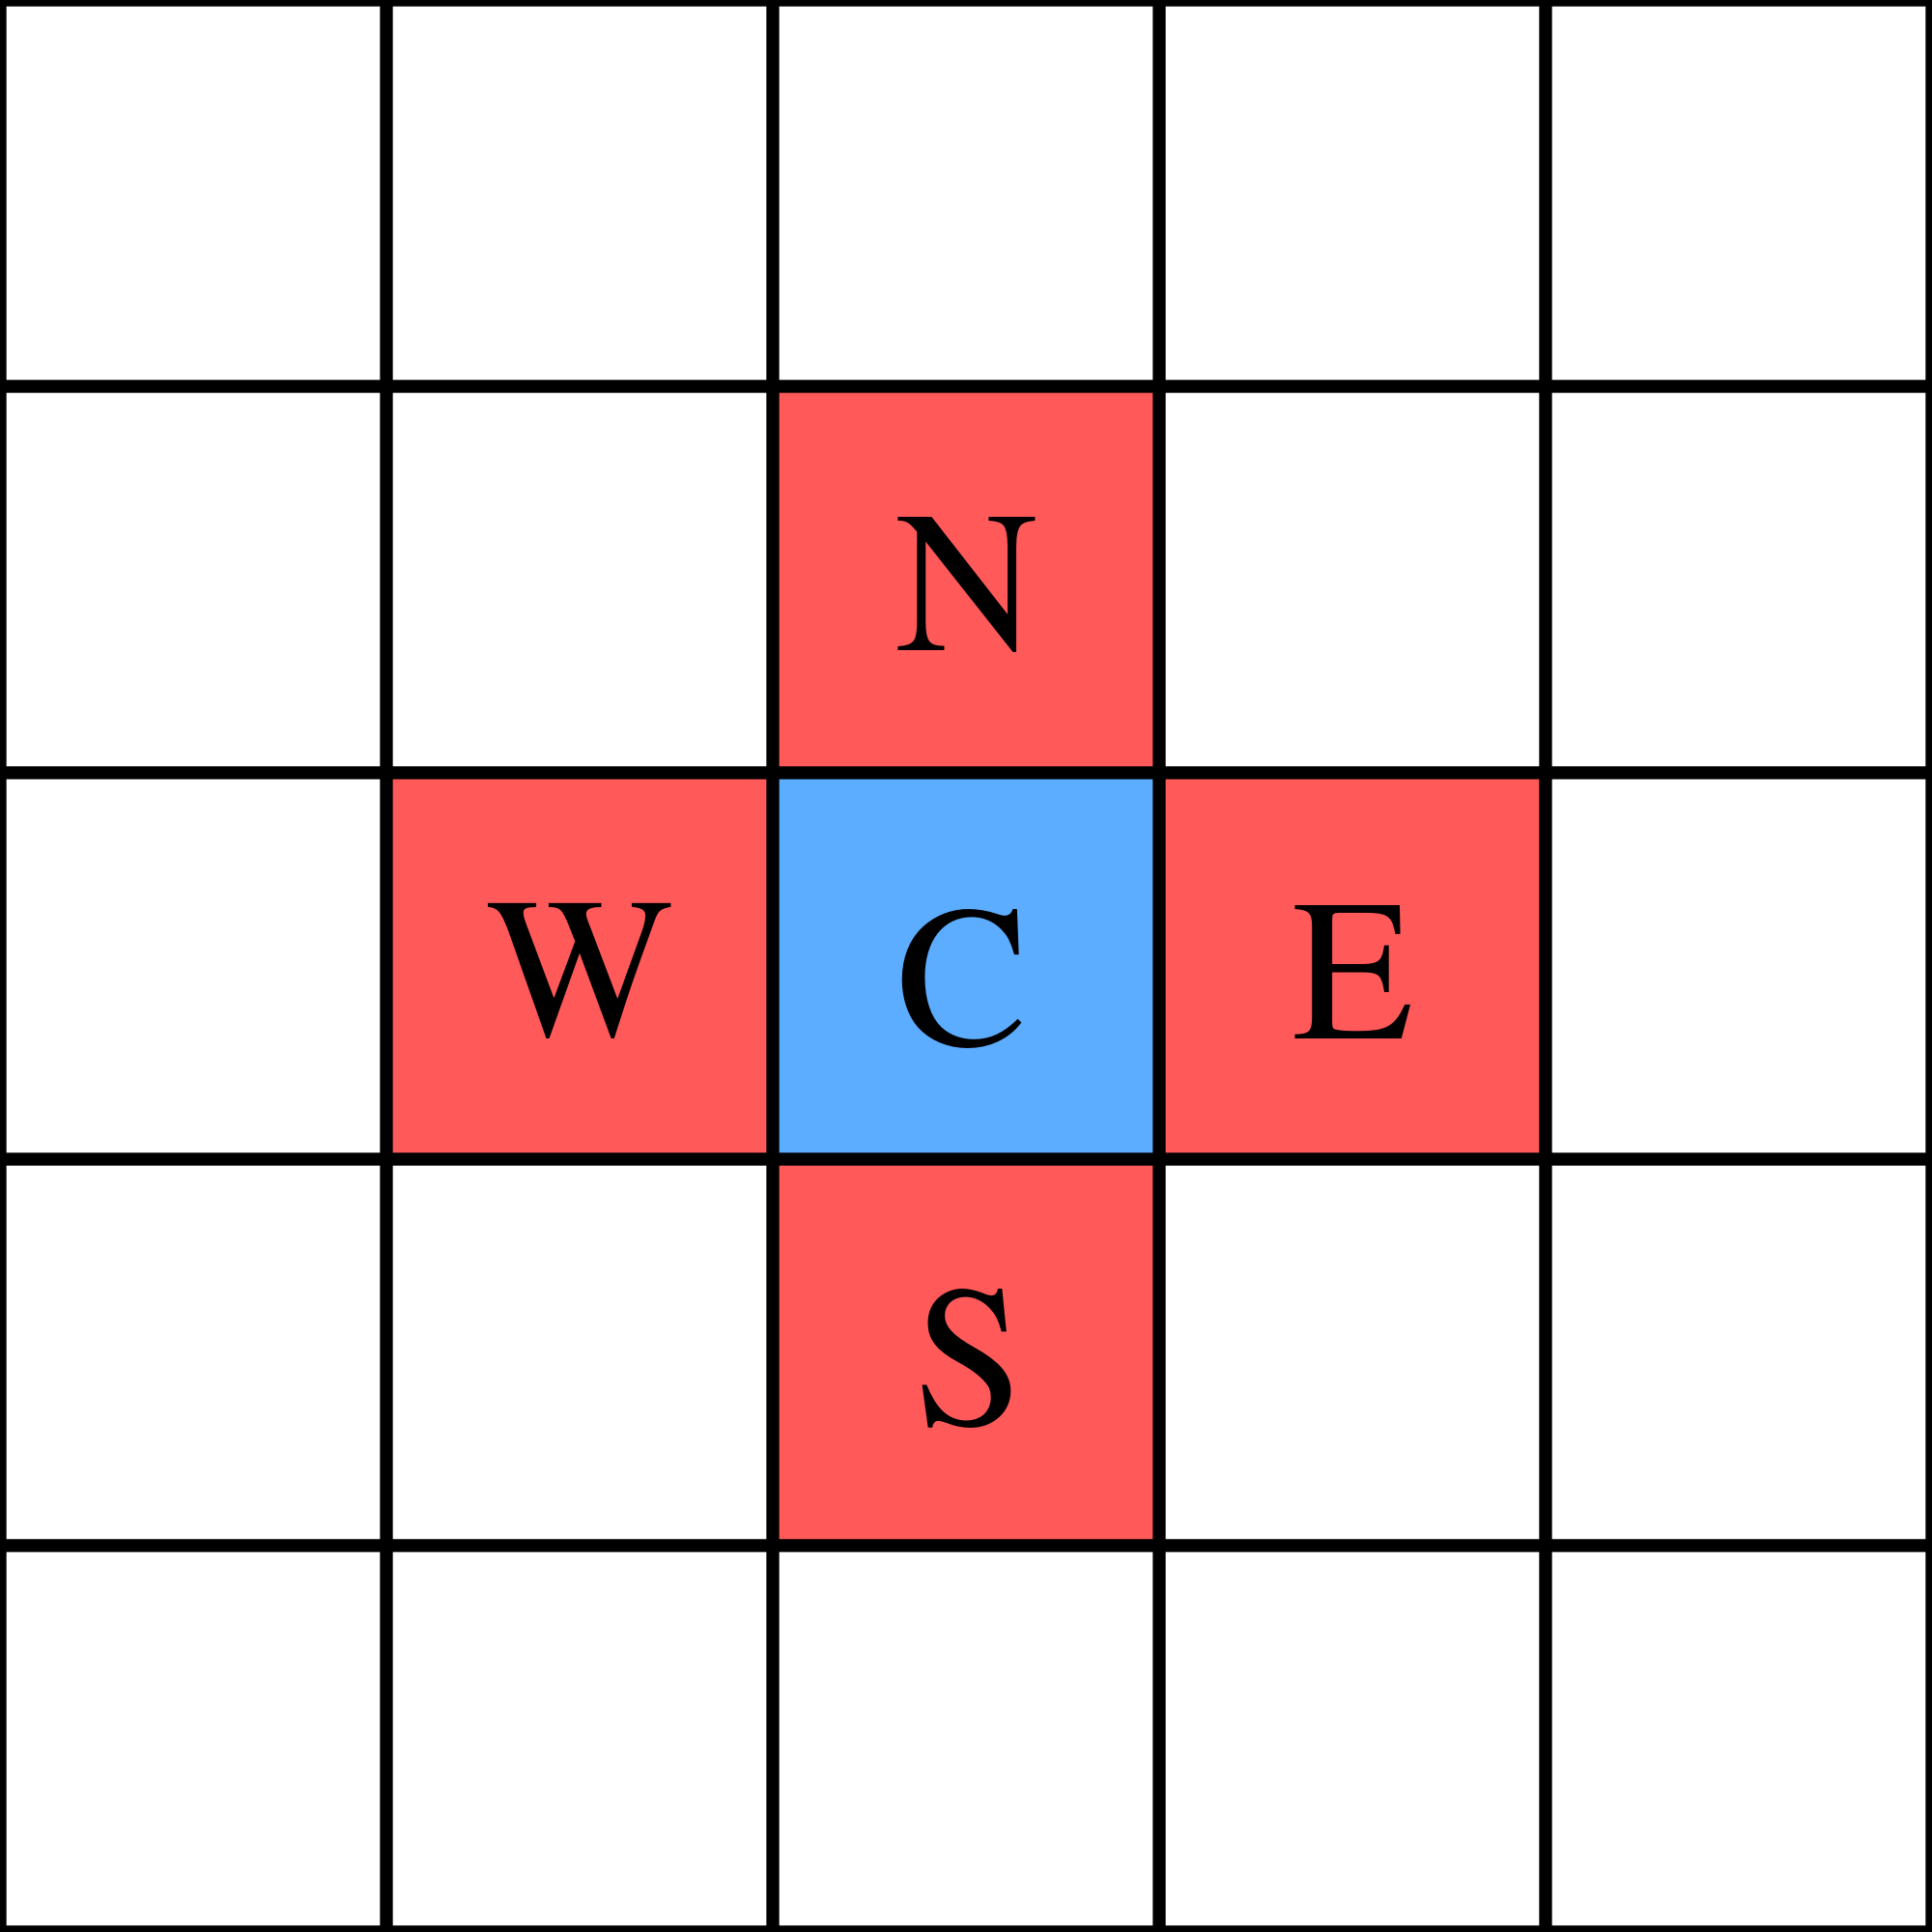
\includegraphics[width=\linewidth]{neumans.png}
    \caption{von Neuman's neighborhood}
    \end{subfigure}
\hfill
    \begin{subfigure}[t]{0.40\textwidth}\centering
    \centering
        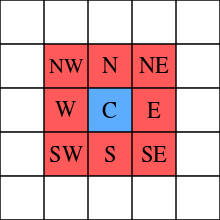
\includegraphics[width=\linewidth]{Moores.png}
    \caption{Moore's neighborhood}
    \end{subfigure}
~
\caption{Possible neighborhoods. (a) A von Neuman's where each node has four neighbors.
(b) Moore's where each node has eight neighbors.}
\label{fig:neighborhood}
\end{figure}

Some further work address the spatial topology in a variate of graphs (ref.).
This dissertation will also follow this approach. Szabo and Fáth dealt with
numerous graphs such as, lattices , small- world, scale free graphs and evolving
networks. We will consider a spatial topology to be any given graph random or
not where the players are the nodes and only interact - play other nodes that are
linked to by an edge. Furthermore, we will conduct a tournament a point out
any significant result.

Another disadvantage of the aforementioned work is that lacked in ways of
reproducing their tournaments.  Due the work done by Axelrod library  (ref.). An
open source python Package which allow us to easily held our experiment.
As it allow to reproduce an IPD tournament and chose bewteen 131 strategies
already given by the library.  Code written for the purpose of this dissertation
has been contributed to the library: see [you'll put your PR urls here].

\section{Structure of Dissertation}
This dissertation is organized into 7 Chapters. Proceeding this introduction:
\begin{itemize}
  \item In Chapter 2 we review previous literature dedicated to the PD/IPD
        and tournaments that have been conducted, different topologies and evolution.
\end{itemize}
